
\documentclass{standalone}
\usepackage{tkz-fct}
\usepackage{tkz-euclide}
\usepackage{color}
\renewcommand*\familydefault{\sfdefault}
\usepackage{sansmath}
\usepackage{amsmath}
\sansmath
\definecolor{gray75}{gray}{0.75}
\begin{document}
 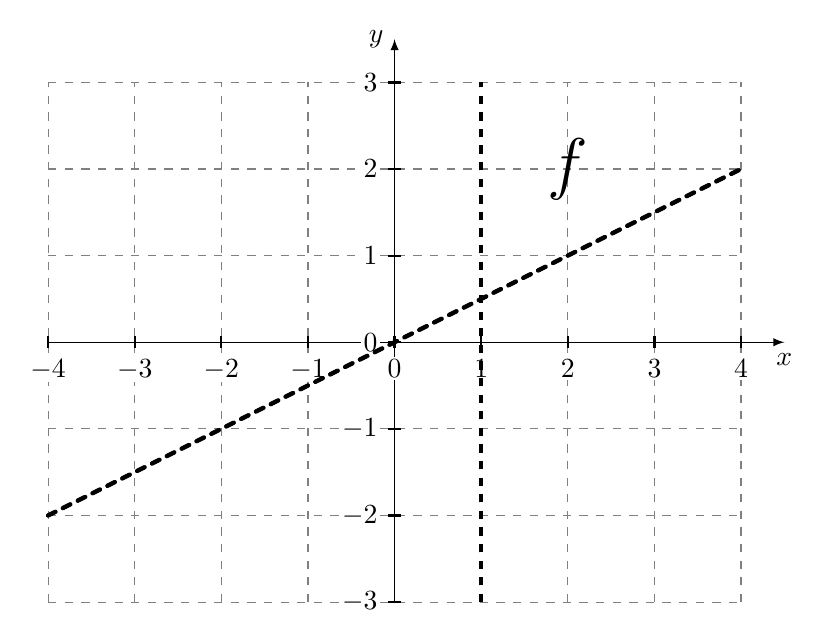
\begin{tikzpicture}[scale=1.1]
   \tkzInit[xmax=4.0,ymax=3.0,xmin=-4.0 ,ymin=-3.0]
   \begin{scope}[dashed]
     \tkzGrid
   \end{scope}
   \tkzDrawX[label={$x$}]
   \tkzDrawY[label={$y$}]
   \tkzLabelX
   \tkzLabelY
   \tkzFctPar[line width=2pt,samples=400,domain=0:1]{((8935141660703067*t**3 - 40177633346264751*t**2 + 53580345837319344*t - 18014398509481984)/4503599627370496)}{(-(448108162923365*t**3 + 7134751336557687*t**2 - 6462589092172641*t + 2257429313219461)/1125899906842624)}
\tkzFctPar[line width=2pt,samples=400,domain=0:1]{((2666130979403333*t**3 + 3988333619780829*t**2 + 10862849324172*t + 2341871806232658)/2251799813685248)}{(-(1792432651693457*t**3 - 23382189400472613*t**2 + 26070838378012800*t - 13510798882111488)/4503599627370496)}


                \tkzDefPoint(-4.0,-2.0){A}

                \tkzDefPoint(4.0,2.0){B}

                \tkzDrawSegment[style=dashed,line width = 1.5pt](A,B)

                \tkzVLine[style=dashed,line width = 1.5pt]{1.0}

                \tkzDefPoint(-4.0,-2.0){A}

                \tkzDefPoint(4.0,2.0){B}

                \tkzDrawSegment[style=dashed,line width = 1.5pt](A,B)

                \tkzVLine[style=dashed,line width = 1.5pt]{1.0}



   \tkzText(2,2){\Huge$f$}

\end{tikzpicture}
\end{document}
